%---------------------------------------------------------------------------%
\lecture{Research Presentation}{lec_present_result}
%---------------------------------------------------------------------------%
\section{Algoritmi}
%---------------------------------------------------------------------------%
\begin{frame}[fragile]
\frametitle{Algoritmi scelti}
\begin{itemize}
    \item Supervisionato: \textbf{Decision Tree} 
    \item Non Supervisionato: \textbf{K-Means} 
\end{itemize}
\end{frame}

%---------------------------------------------------------------------------%
\begin{frame}[fragile]
\frametitle{Decision Tree}
\begin{minipage}{0.45\textwidth}
\begin{figure}
    \centering
    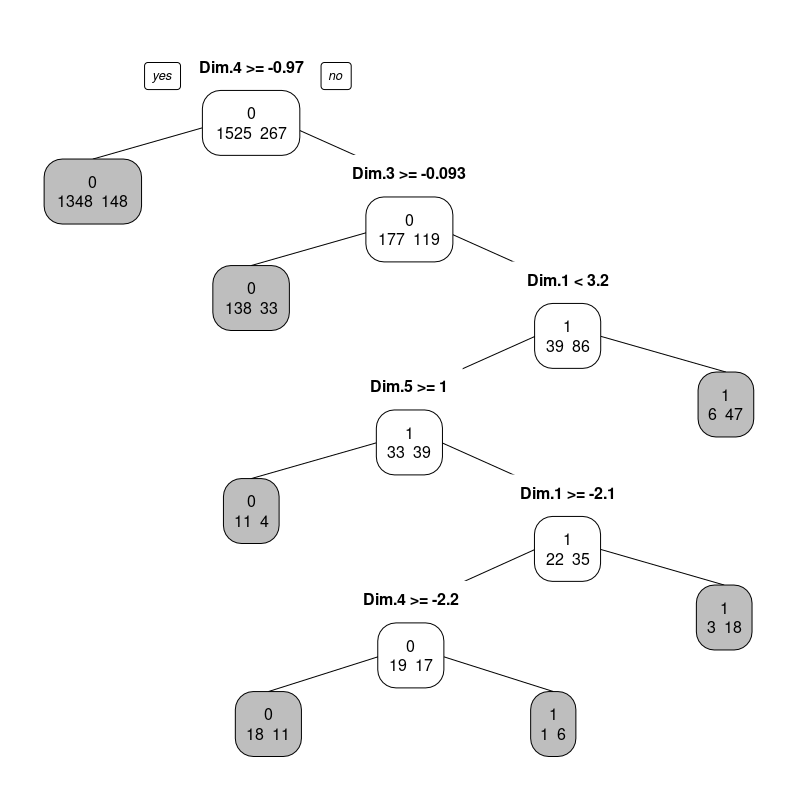
\includegraphics[width=0.8\textwidth]{Img/decision tree/D-TREE001.png}
    \caption{Decision Tree}
    \label{fig:DTREE1}
\end{figure}
\end{minipage}%
\hspace{2em}
\begin{minipage}{0.45\textwidth}

\begin{table}[h!]
\centering
\begin{tabular}{ll}
\multicolumn{2}{l}{\textbf{Positive Class:} 1} \\
\textbf{Accuracy:} 0.8348 & \textbf{Precision:} 0.1194\\
\textbf{Recall:} 0.3478 & \textbf{F-Measure:} 0.1777
\end{tabular}
\end{table}
\end{minipage}%
\end{frame}

%---------------------------------------------------------------------------%
\begin{frame}[fragile]
\frametitle{Decision Tree: Riduzione Overfitting}
\begin{minipage}{0.45\textwidth}
\begin{figure}
    \centering
    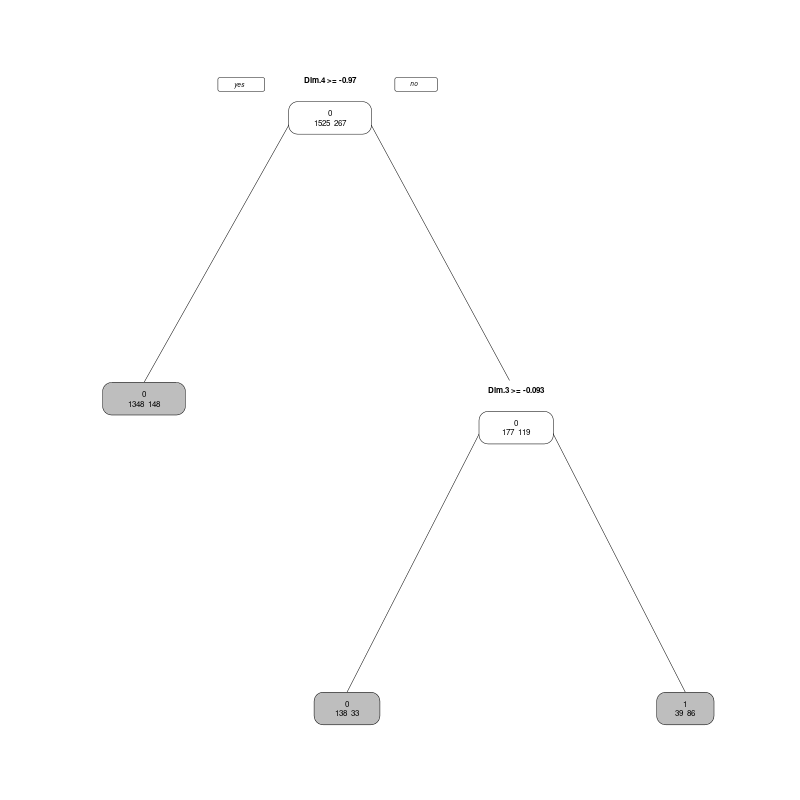
\includegraphics[width=\textwidth]{Img/decision tree/D-TREE002.png}
    \caption{Decision Tree semplice}
    \label{fig:DTREE2}
\end{figure}
\end{minipage}%
\hspace{2em}
\begin{minipage}{0.45\textwidth}

\begin{table}[h!]
\centering
\begin{tabular}{ll}
\multicolumn{2}{l}{\textbf{Positive Class:} 1} \\
\textbf{Accuracy:} 0.8147 & \textbf{Precision:} 0.2777\\
\textbf{Recall:} 0.1492 & \textbf{F-Measure:} 0.1941
\end{tabular}
\end{table}
\end{minipage}%
\end{frame}

%---------------------------------------------------------------------------%
\begin{frame}[fragile]
\frametitle{K-Means: Elbow Method}
\begin{figure}[H]
   \begin{minipage}{0.48\textwidth}
     \centering
     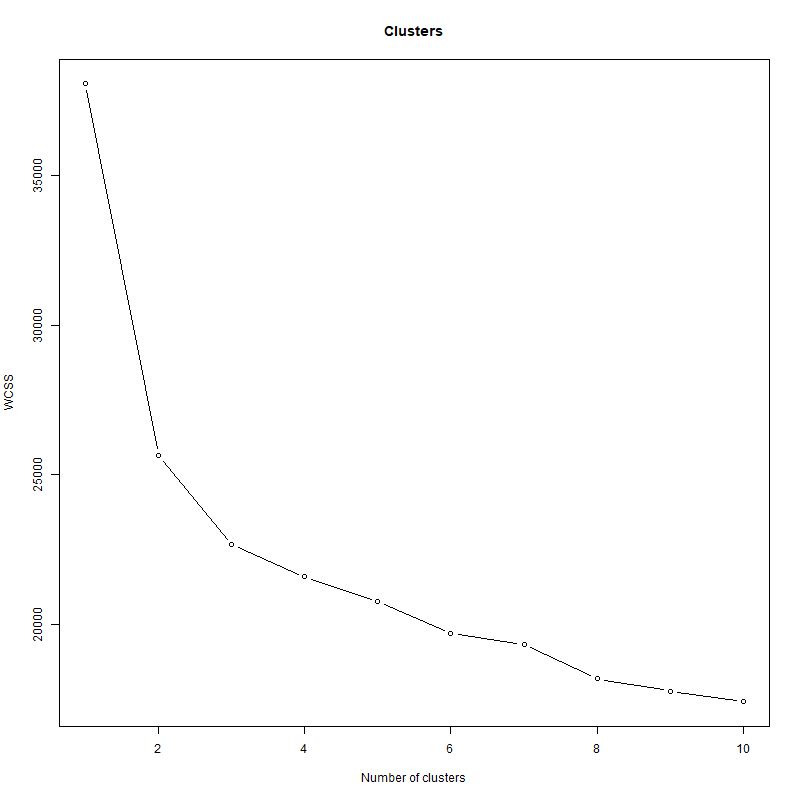
\includegraphics[width=0.8\linewidth]{Img/KMEANS001.png}
     \caption{Elbow Method effettuato manualmente}\label{fig:Elbow1}
   \end{minipage}\hfill
   \begin{minipage}{0.48\textwidth}
     \centering
     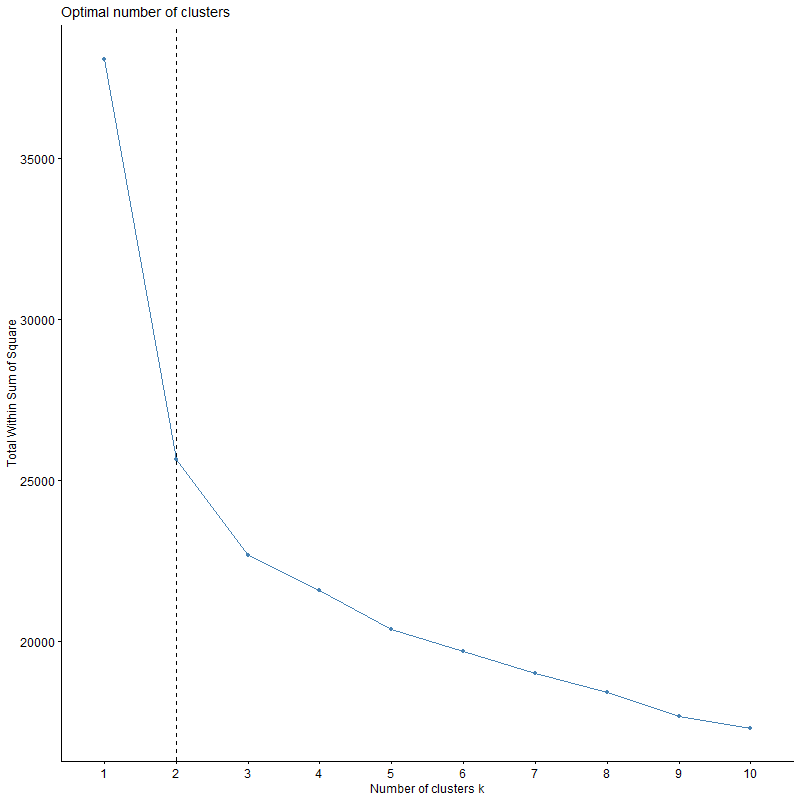
\includegraphics[width=0.8\linewidth]{Img/KMEANS002.png}
     \caption{Elbow Method effettuato automaticamente dal metodo $fviz\_nbclust$}\label{fig:Elbow2}
   \end{minipage}
\end{figure}
\end{frame}
%---------------------------------------------------------------------------%
\begin{frame}[fragile]
\frametitle{K-Means: Silhouette}
\begin{minipage}{0.45\textwidth}
\begin{figure}[H]
        \centering
     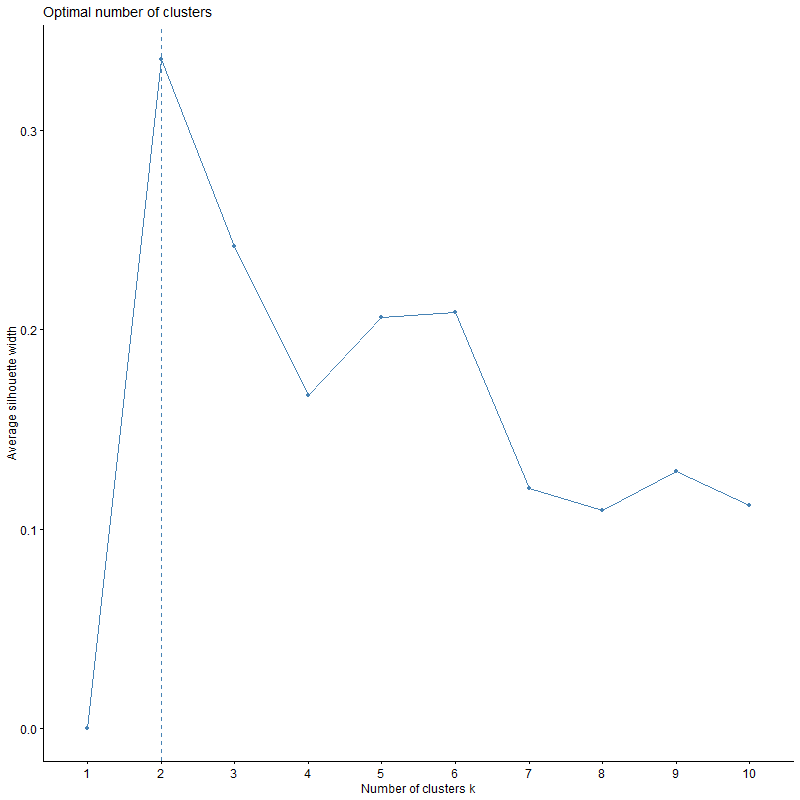
\includegraphics[width=0.7\linewidth]{Img/KMEANS004.png}
     \caption{Silhouette effettuata automaticamente dal metodo $fviz\_nbclust$}\label{fig:Silhouette2}
\end{figure}
\end{minipage}%
\hspace{2em}
\begin{minipage}{0.45\textwidth}
\begin{tabular}{|p{\textwidth}}
Sia \textbf{Elbow Method} che \textbf{Silhouette} mostrano un numero di clusters ottimo pari a due.
\end{tabular}
\end{minipage}%
\end{frame}
%---------------------------------------------------------------------------%
\begin{frame}[fragile]
\frametitle{K-Means: Algoritmo}
\begin{figure}[H]
   \begin{minipage}{0.48\textwidth}
     \centering
         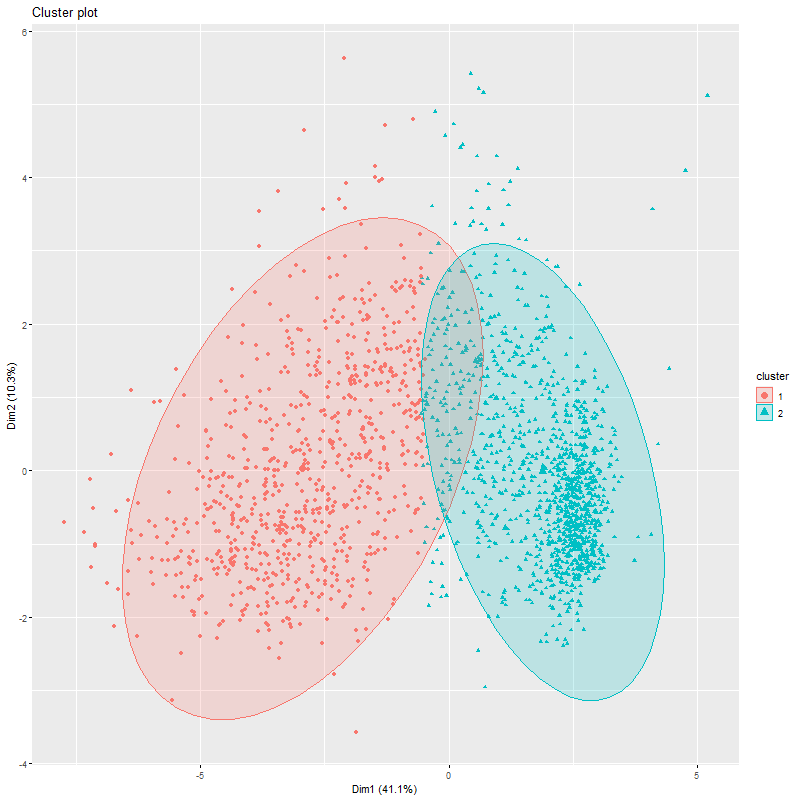
\includegraphics[width=0.8\textwidth]{Img/KMEANS005.png}
    \caption{Partizionamento in clusters dei dati}
    \label{fig:clusters}
   \end{minipage}\hfill
   \begin{minipage}{0.48\textwidth}
     \centering
     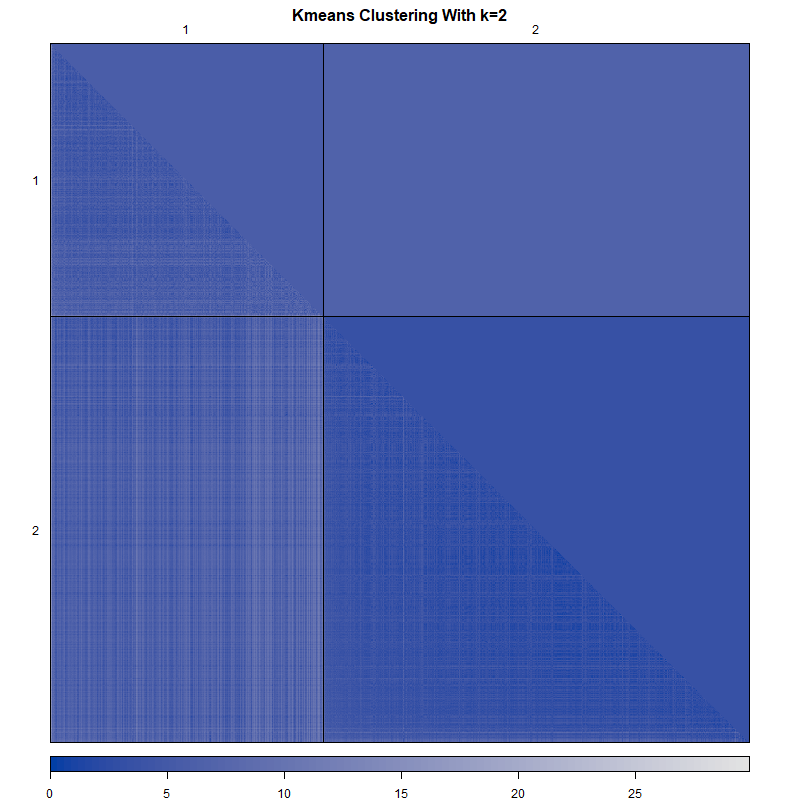
\includegraphics[width=0.8\linewidth]{Img/KMEANS006.png}
     \caption{Dissimilarity matrix}\label{fig:dissimilaritymatrix}
   \end{minipage}
\end{figure}
\end{frame}
%---------------------------------------------------------------------------%
\begin{frame}[fragile]
\frametitle{K-Means: Analisi Wines}
\begin{minipage}{0.45\textwidth}
\begin{figure}[H]
        \centering
     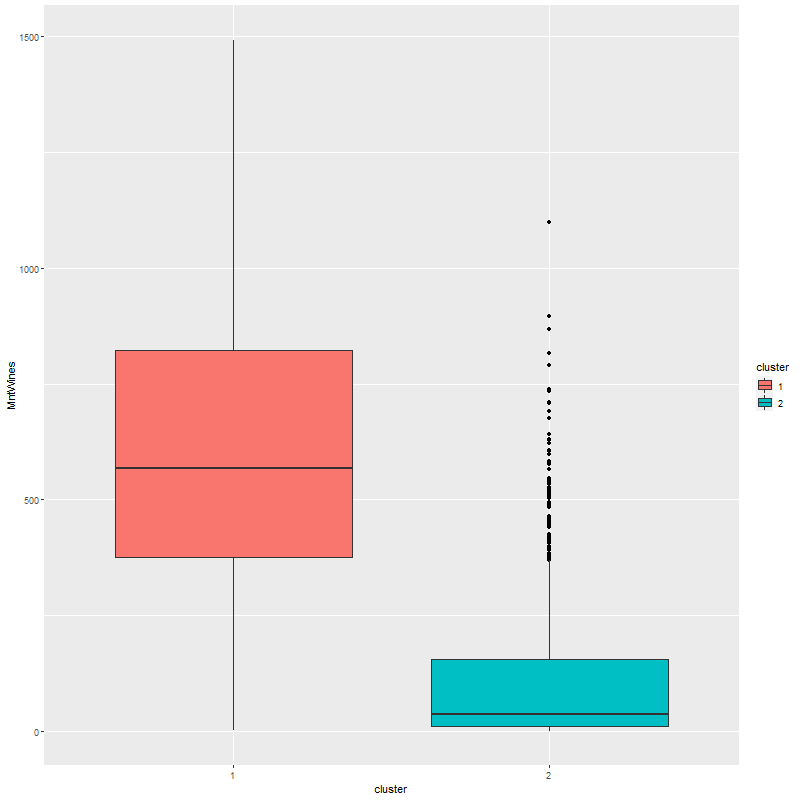
\includegraphics[width=0.8\linewidth]{Img/KMEANS009.png}
      \caption{BoxPlot della variabile Wines in relazione al numero di cluster}
    \label{fig:winesKmeansBoxPlot}
\end{figure}
\end{minipage}%
\hspace{2em}
\begin{minipage}{0.45\textwidth}
\begin{itemize}
    \item Spesa maggiore di vini per i \textit{customers} all'interno del primo cluster
    \item La maggior parte dei clienti all'interno del secondo cluster non ha acquistato vini negli ultimi due anni
\end{itemize}
\end{minipage}%
\end{frame}
%---------------------------------------------------------------------------%
\begin{frame}[fragile]
\frametitle{K-Means: Analisi Income}
\begin{minipage}{0.45\textwidth}
\begin{figure}[H]
        \centering
    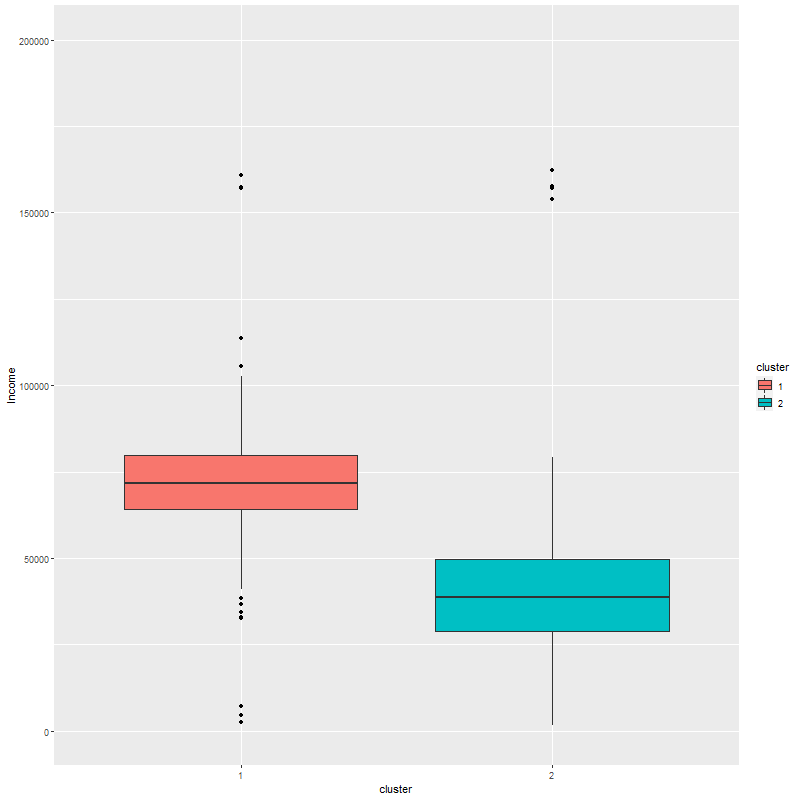
\includegraphics[width=0.8\textwidth]{Img/KMEANS012.png}
    \caption{BoxPlot della variabile income in relazione al numero di cluster}
    \label{fig:incomeKmeansBoxPlot}
\end{figure}
\end{minipage}%
\hspace{2em}
\begin{minipage}{0.45\textwidth}
\begin{itemize}
    \item Gli elementi del primo raggruppamento godono di un reddito medio maggiore rispetto ai secondi
    \item La maggior parte degli elementi nel secondo cluster possiedono un il reddito inferiore alla media.
\end{itemize}
\end{minipage}%
\end{frame}
%---------------------------------------------------------------------------%
\begin{frame}[fragile]
\frametitle{K-Means: Analisi Total\_spent}
\begin{minipage}{0.45\textwidth}
\begin{figure}[H]
        \centering
    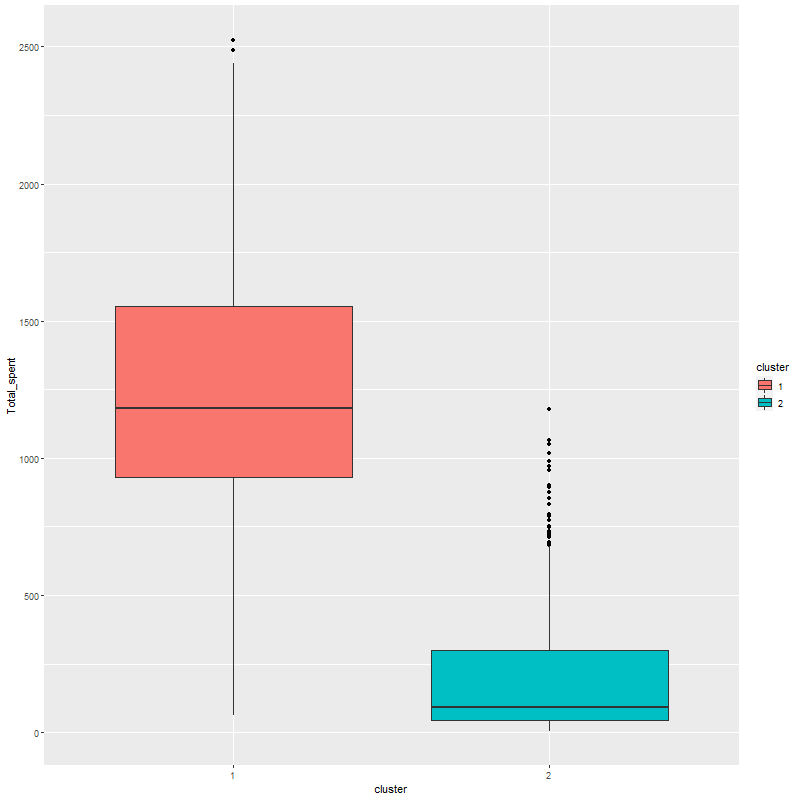
\includegraphics[width=0.8\textwidth]{Img/KMEANS015.png}
    \caption{BoxPlot della variabile Total\_spent in relazione al numero di cluster}
    \label{fig:TotalSpentKmeansBoxPlot}
\end{figure}
\end{minipage}%
\hspace{2em}
\begin{minipage}{0.45\textwidth}
\begin{itemize}
    \item I compratori del secondo cluster generalmente spendono molto meno denaro rispetto a quelli del primo.
\end{itemize}
\end{minipage}%
\end{frame}
%---------------------------------------------------------------------------%
\begin{frame}[fragile]
\frametitle{K-Means: Analisi NumCatalogPurchases}
\begin{minipage}{0.45\textwidth}
\begin{figure}[H]
        \centering
    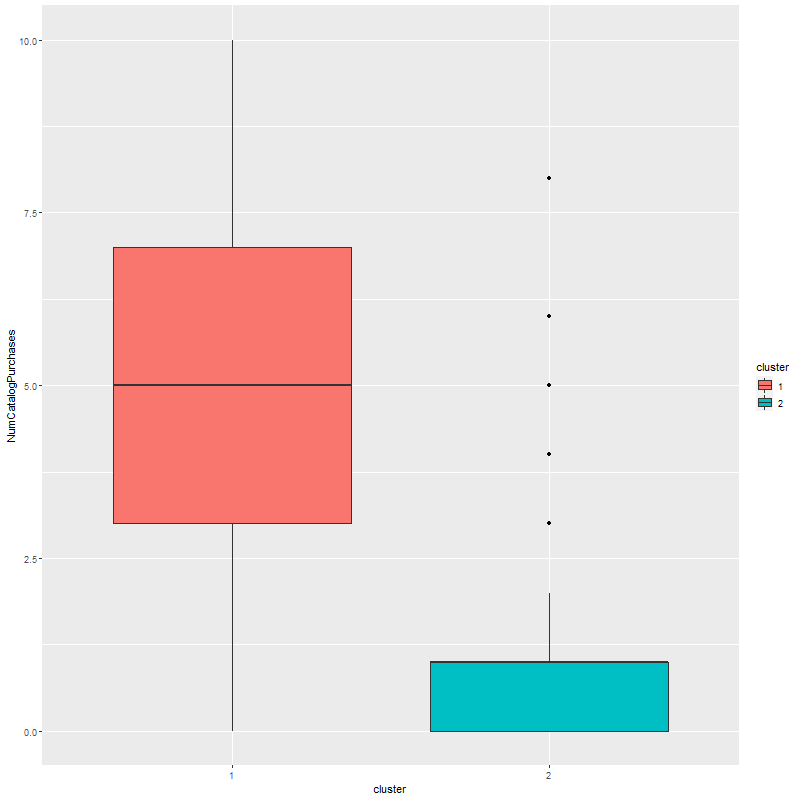
\includegraphics[width=0.8\textwidth]{Img/KMEANS018.png}
    \caption{BoxPlot della variabile NumCatalogPurchases in relazione al numero di cluster}
    \label{fig:NumCatalogPurchasesKmeansBoxPlot}
\end{figure}
\end{minipage}%
\hspace{2em}
\begin{minipage}{0.45\textwidth}
\begin{itemize}
    \item I clienti del secondo cluster effettuano compere sul catalogo generalmente in quantità minore rispetto a quelli del primo.
    \item I clienti del secondo cluster acquistano mediamente 5 prodotti dal catalogo.
\end{itemize}
\end{minipage}%
\end{frame}
%---------------------------------------------------------------------------%
\begin{frame}[fragile]
\frametitle{K-Means: Analisi NumCatalogPurchases}
\begin{minipage}{0.45\textwidth}
\begin{figure}[H]
        \centering
    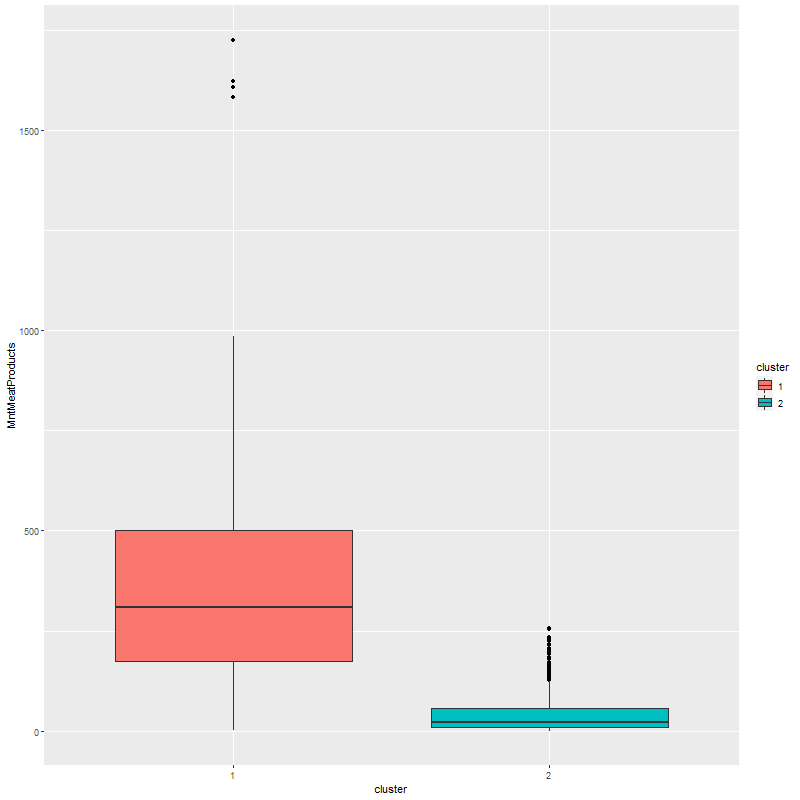
\includegraphics[width=0.8\textwidth]{Img/KMEANS021.png}
    \caption{BoxPlot della variabile MntMeatProducts in relazione al numero di cluster}
    \label{fig:MntMeatProductsKmeansBoxPlot}
\end{figure}
\end{minipage}%
\hspace{2em}
\begin{minipage}{0.45\textwidth}
\begin{itemize}
    \item Correlazione con Total\_spent
    \item Gli acquirenti del secondo raggruppamento tendano a spendere generalmente di meno rispetto a quelli del primo
\end{itemize}
\end{minipage}%
\end{frame}


